\chapter{AdaptaMaterialEscolar 2.0}
\label{cap:AdaptaMaterialEscolar2.0}
En este capítulo explicaremos la obtención de requisitos y su priorización en la Sección \ref{cap:requisitos}. También se describirá la iteración competitiva para el diseño de la aplicación en la Sección \ref{disenyoDeLaAplicacion}.

\section{Requisitos}
\label{cap:requisitos}

Lo primero que hicimos fue analizar la memoria de AdaptaMaterialEscolar 1.0 extrayendo las funcionalidades que faltaban por implementar y los resultados de la evaluación que se realizó. Tras este análisis surgieron una seria de cambios y nuevas funcionalidades. Agrupamos dichas funcionalidades en tres grupos: formato, ejericios y auxiliar. Quedando las funcionalidades agrupadas de la siguiente manera:
\\

Formato: 
\begin{itemize}
  \item Añadir encabezado al texto: el usuario elijará un encabezado y se le añadirá al CKEditor.
  \item Añadir un tipo de fuente escolar: incluir en los tipos de fuentes la escolar.
  \item Añadir una leyenda de colores con la categoría de cada tipo: crear leyenda de colores según unas características.
  \item Añadir leyenda de colores para el tema de cada asignatura: crear una leyenda según el color del borde de la hoja asignada a cada asignatura.
  \item Añadir ejercicios de matemáticas con cuadrícula para escribir los números: crear una hoja de cuadrículas para los ejercicios de matemáticas.
  \item Añadir la alternativa de añadir doble pauta: en vez de renglones de una única línea, se podrá crear una hoja con doble pauta, para determinar el tamaño de la letra del alumno.
  \item Estandarizar formato para títulos e índices del temario: escoger un formato para el editable.
  \item Enumerar ejercicios de forma automática: establecer un orden numérico para los ejercicios.
\end{itemize}
Ejercicios:
\begin{itemize}
  \item Ejercicios de relacionar contenido mediante flechas: generar un ejercicio para relacionar conceptos.
  \item Añadir ejercicios de cálculo con huecos a rellenar por el alumno: espacios en blanco para que el alumno pueda rellenarlos con el contenido adecuado.
  \item Añadir ejercicios con espacio para dibujar: amplio hueco en blanco con el fin de que el alumno pueda dibujar.
  \item Ejercicios de completar los espacios en blanco en tablas y esquemas: dado una tabla o esquema se establen espacios en blanco para que el alumno los rellene con el contenido adecuado.
\end{itemize}
Auxiliar:
\begin{itemize}
  \item Generar un resumen a partir de un texto: se crea un resumen a partir de un texto.
  \item Exportar el documento a formato Word para hacer modificaciones: exportar un docuemnto PDF a Word.
  \item Añadir un pictotraductor como funcionalidad: dado una frase genera sus respectivos pictogramas.
  \item Añadir imágenes buscando una palabra: a partir de una palabra se busca su respectiva imagen en las bases de datos de imágenes libres.
  \item Sustituir una palabra por una imagen: una palabra se reemplazará por una imagen.
  \item Crear una herramienta de recorte de imágenes para el texto original: añadir una herramienta que recorte imágenes del texto original.
  \item Crear tablas que organicen el temario y/o las actividades, seleccionando contenido: seleccionando el contenido crea una tabla.
  \item Crear esquemas que faciliten la visualización: añadir un esquema para visualizar fácilmente los contenidos.
\end{itemize}
Tras haber analizado en detalle las funcionalidades anteriores hemos encontrado que varias funciones ya están realizadas y otras no se van a implementar por falta de información. A continuación, especificamos las funciones realizadas, las funciones que no aportan información suficiente y las que realizaremos.

Funciones realizadas:
  \begin{itemize}
    \item Añadir encabezado al texto: el usuario elijará un encabezado y se le añadirá al CKEditor.
    \item Enumerar ejercicios de forma automática: establecer un orden numérico para los ejercicios.
  \end{itemize}
Funciones sin información suficiente:
\begin{itemize}
  \item Añadir imágenes buscando una palabra: a partir de una palabra se busca su respectiva imagen en las bases de datos de imágenes libres.
  \item Sustituir una palabra por una imagen: una palabra se reemplazará por una imagen.
  \item Crear una herramienta de recorte de imágenes para el texto original: añadir una herramienta que recorte imágenes del texto original.
  \item Crear tablas que organicen el temario y/o las actividades, seleccionando contenido: seleccionando el contenido crea una tabla.
  \item Crear esquemas que faciliten la visualización: añadir un esquema para visualizar fácilmente los contenidos.
  \item Ejercicios de completar los espacios en blanco en tablas y esquemas: dado una tabla o esquema se establen espacios en blanco para que el alumno los rellene con el contenido adecuado.
\end{itemize}

Por lo tanto, las fuciones a implementar son las que se muestran a continuación:


\begin{itemize}
  \item Generar un resumen a partir de un texto: se crea un resumen a partir de un texto.
  \item Exportar el documento a formato Word para hacer modificaciones: exportar un docuemnto PDF a Word.
  \item Añadir un pictotraductor como funcionalidad: dado una frase genera sus respectivos pictogramas.
  \item Ejercicios de relacionar contenido mediante flechas: generar un ejercicio para relacionar conceptos.
  \item Añadir un tipo de fuente escolar: incluir en los tipos de fuentes la escolar.
  \item Añadir una leyenda de colores con la categoría de cada tipo: crear leyenda de colores según unas características.
  \item  Añadir ejercicios de cálculo con huecos a rellenar por el alumno: espacios en blanco para que el alumno pueda rellenarlos con el contenido adecuado.
  \item  Añadir ejercicios con espacio para dibujar: amplio hueco en blanco con el fin de que el alumno pueda dibujar.
  \item Añadir leyenda de colores para el tema de cada asignatura: crear una leyenda según el color del borde de la hoja asignada a cada asignatura.
  \item Añadir ejercicios de matemáticas con cuadrícula para escribir los números: crear una hoja de cuadrículas para los ejercicios de matemáticas.
  \item Añadir la alternativa de añadir doble pauta: en vez de renglones de una única línea, se podrá crear una hoja con doble pauta, para determinar el tamaño de la letra del alumno.
  \item Estandarizar formato para títulos e índices del temario: escoger un formato para el editable.

\end{itemize}                                               

\section{Diseño de la apliación}
\label{disenyoDeLaAplicacion}
Para el diseño de la aplicación web hemos realizado una iteración competitiva. Cada integrante del grupo ha proporcionado un diseño de la apliación como se muestra en las figuras \ref{IteracionCompetitiva1}, \ref{IteracionCompetitiva2}, \ref{IteracionCompetitiva3} y \ref{IteracionCompetitiva4}.
Una vez que cada integrante ha explicado su diseño, hemos cogido lo mejor de cada uno quedando la aplicación de la siguiente manera \ref{diseño_final}.


\begin{figure}[ht!]
    \centering
    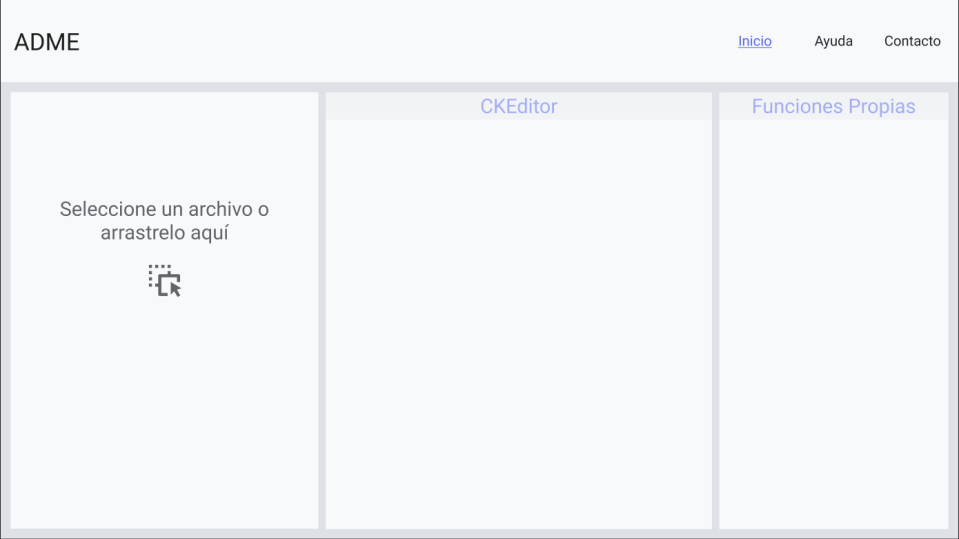
\includegraphics[scale=0.3]{Diseño/IteracionCompetitiva1}
    \caption{Diseño aplicación iteración competitiva 1.}
    \label{IteracionCompetitiva1}
\end{figure}
\begin{figure}[ht!]
    \centering
    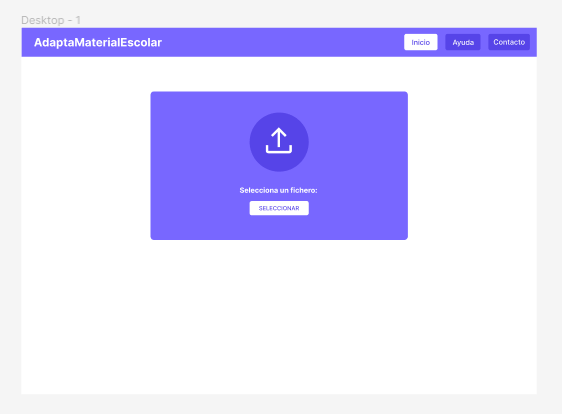
\includegraphics[scale=0.5]{Diseño/IteracionCompetitiva2}
    \caption{Diseño aplicación iteración competitiva 2.}
    \label{IteracionCompetitiva2}
\end{figure}
\begin{figure}[ht!]
    \centering
    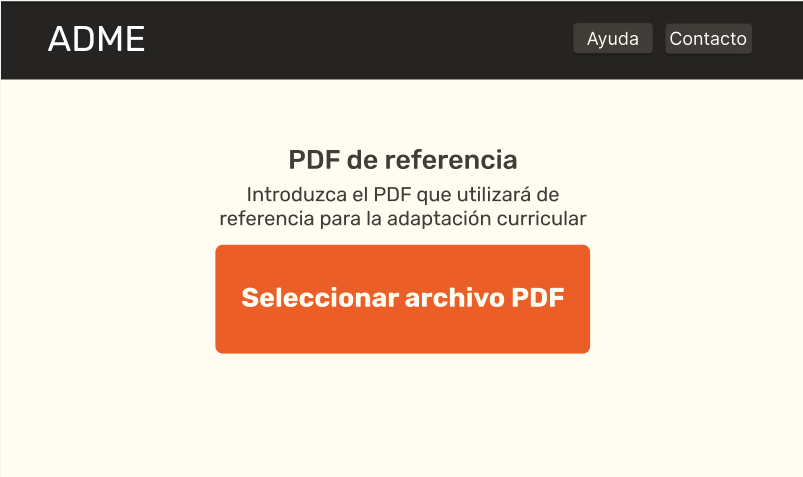
\includegraphics[scale=0.5]{Diseño/IteracionCompetitiva3}
    \caption{Diseño aplicación iteración competitiva 3.}
    \label{IteracionCompetitiva3}
\end{figure}
\begin{figure}[ht!]
    \centering
    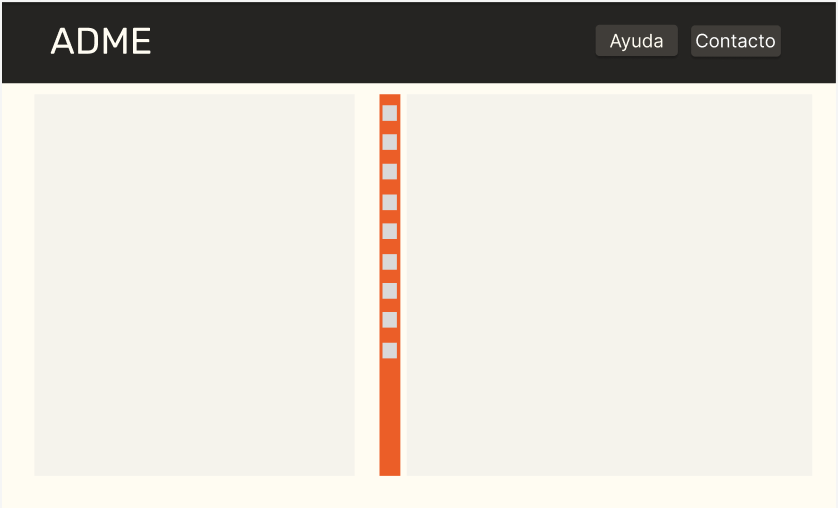
\includegraphics[scale=0.5]{Diseño/IteracionCompetitiva4}
    \caption{Diseño aplicación iteración competitiva 4.}
    \label{IteracionCompetitiva4}
\end{figure}
\begin{figure}[ht!]
  \centering
  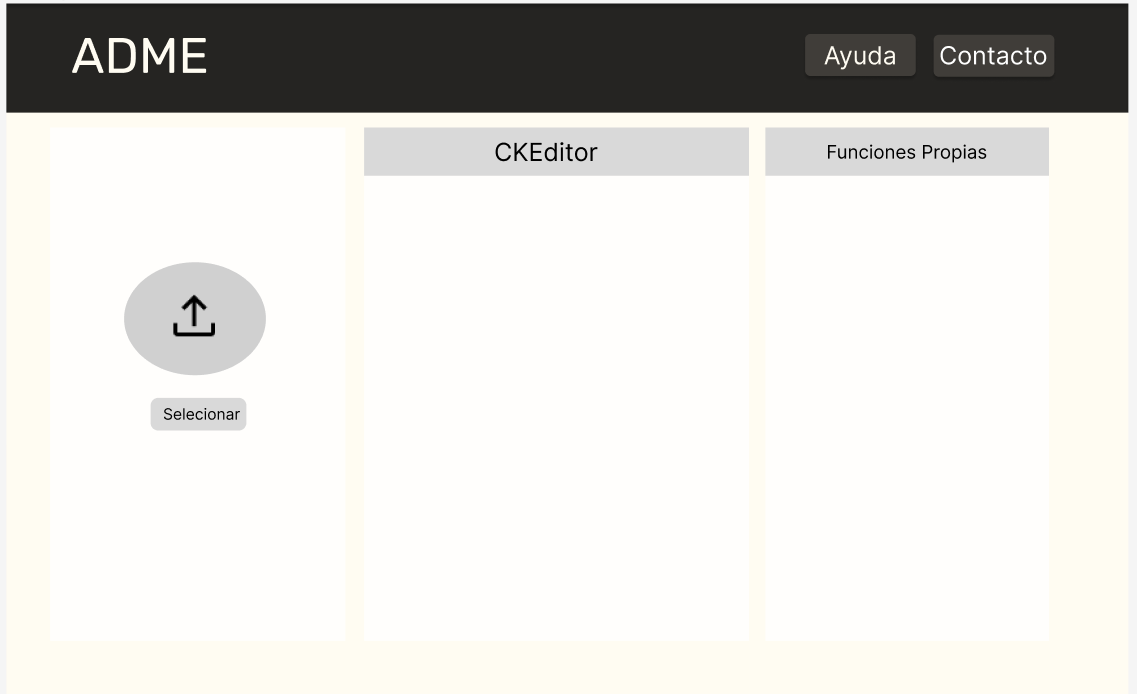
\includegraphics[scale=0.3]{Diseño/Diseño Final}
  \caption{Diseño final aplicación.}
  \label{diseño_final}
\end{figure}
